
\pagebreak
\setauthorname{Martin Usta}
\chapter{Spieleperformance}


\subsection{Einführung}
In jedem Spiel ist es wichtig, dass das Spiel ohne Performanceverluste funktioniert. Die Performance wird von der Spielewelt und ihren Spielobjekten beeinträchtigt. Bei der Spielentwicklung muss sehr oft abgewogen werden ob bestimmte Details ins Spiel implementiert sein müssen. Denn jedes noch so kleine Detail braucht Rechenleistung. In der Spieleentwicklung werden nur selten Spielobjekte wegen des Leistungsverlustes entfernt. Meistens werden diese für das Spiel optimiert.Bei der Spieleentwicklung kann man die Performance anhand von zwei Faktoren optimieren. Ein Faktor betrifft dabei die Spiel-Engine, während der andere Faktor das Modellierungsprogramm betrifft.. %todo: fix text grammar

\subsection{Spielobjekt Optimierung im Grafikprogramm}
Bei den Grafikprogrammen kann vieles gemacht werden um das Spielobjekt performance effizienter zumachen. Wenn ein Gameobjekt erstellt wird, besteht dieses aus Seiten und Flächen. Diese werden auch Polygone genannt. Die Polygon Anzahl bestimmt den Detailgrad des Spielobjekts, das heißt je mehr Polygone das Objekt besitzt desto detailreicher ist es. Wenn ein Objekt viele Polygone besitzt, kann es sein das die Performance im Spiel darunter leidet. Denn sobald sich ein Polygon in der Darstellungsdistanz befindet, wird es berechnet. Um die Anzahl der Polygone niedrig zu halten, werden die Details als "Objekt-Images" gezeichnet. \\\\ %todo: change the ****
Bei dem ersten Prototypen entstand das Problem, dass mehrere Spielobjekte zu viele Polygone hatten. Somit mussten wir die meisten Objekte in unseren Prototypen neu bearbeiten. Dieser Vorgang wird auch als 'Mapping' bezeichnet. %todo: fix the ""
\pagebreak
\subsection{Objekt Mapping}

Bei einem Objekt-Image handelt es sich um ein Bild, welches über das Objekt gelegt wird. Für dieses Verfahren muss erst das Objekt für das Bild \verb+unwrapped+ werden. Dieser Vorgang zerlegt das Objekt in sogenannten Maps.\\\\
In der nächsten Abbildung wird auf der linken Seite eine \verb+unwrapped+ Map von einem Stein gezeigt, der in unseren Prototypen implementiert wird. Auf der rechten Seite ist das 3D-Objekt abgebildet.


\begin{figure}[H]
    \centering
    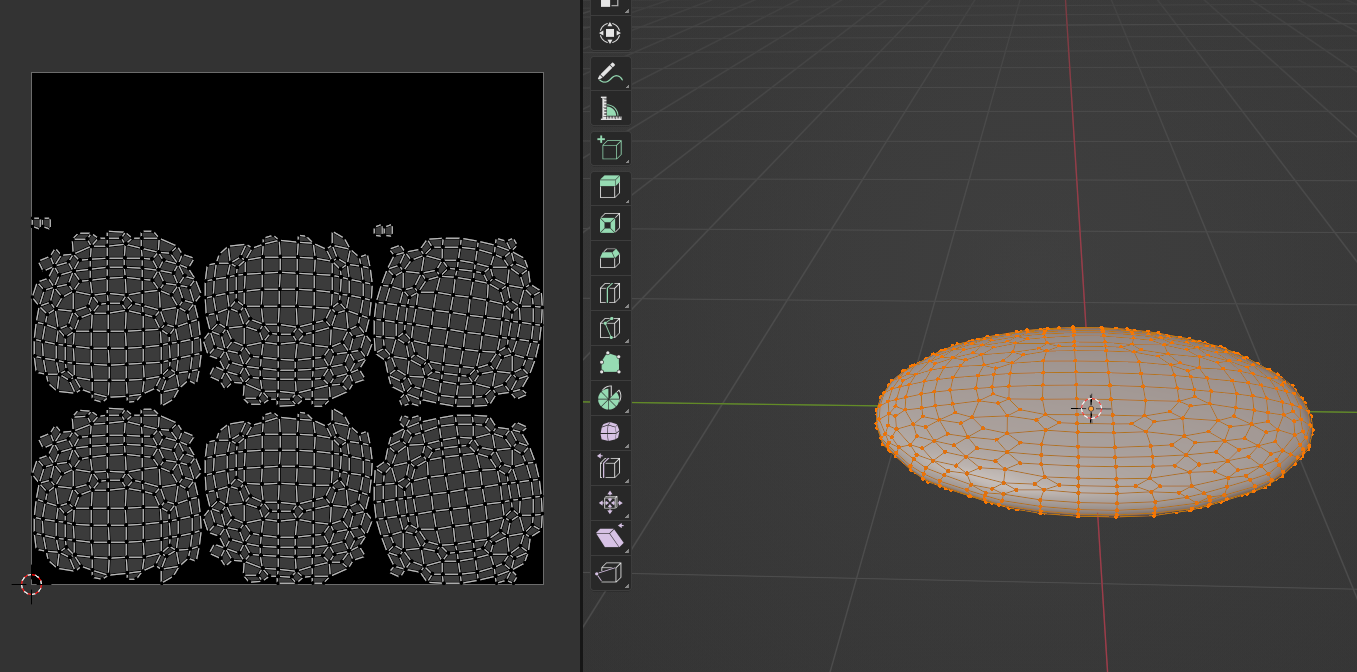
\includegraphics[width=0.8\textwidth]{chapters/11/Images/StoneAndUnwrap.png}
    \caption{Eine Abbildung einer unwrapped map und des Objektes.}
    \label{htl01}
\end{figure}

\noindent Nun könnte man ein Bild unter das entfaltete Mapping legen und damit weiterarbeiten. Auf diesem Bild können nun sämtliche Details eingezeichnet werden. Sobald die Details eingezeichnet wurden, wird das Bild "gebacken". Im folgenden Bild sieht man das Objektbild eines Steins: %todo: maybe rewrite this

\begin{figure}[H]
    \centering
    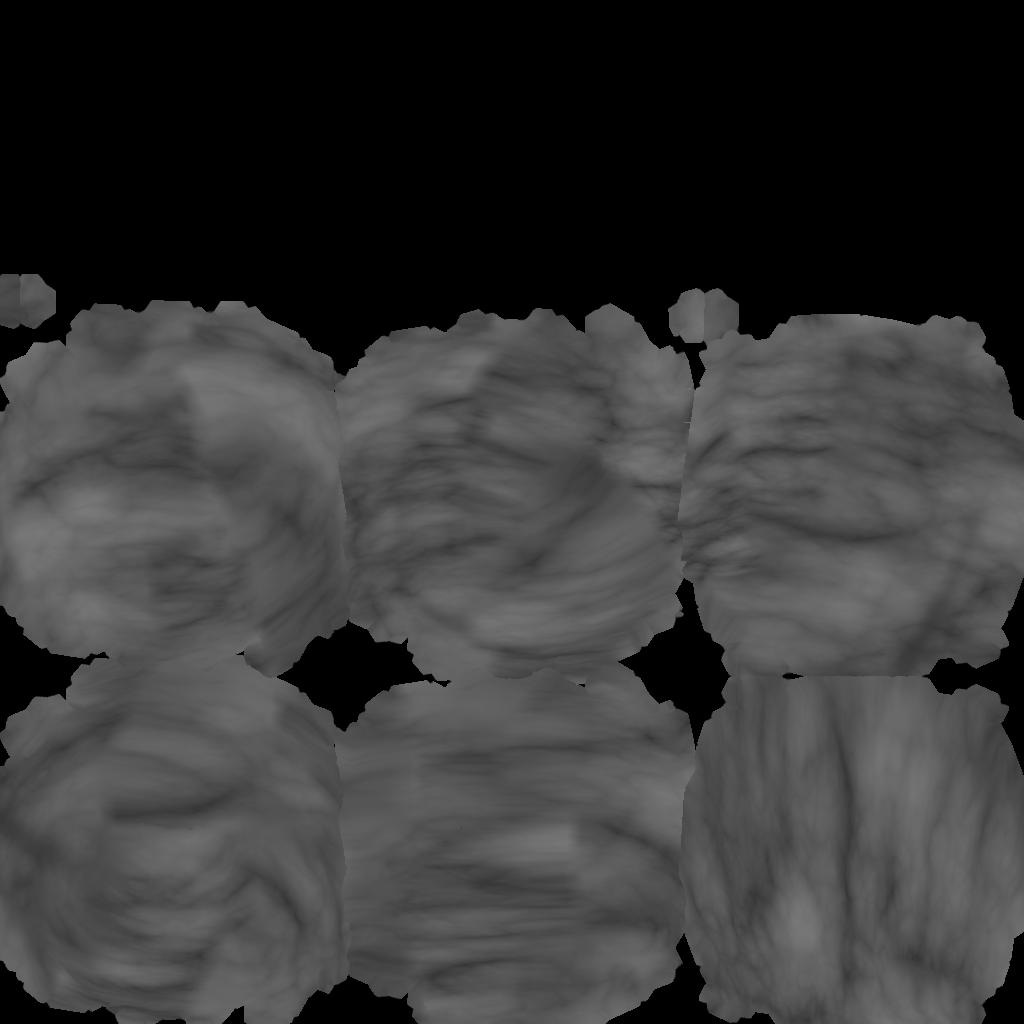
\includegraphics[width=0.4\textwidth]{chapters/11/Images/SteinColor.png}
    \caption{Eine Abbildung einer Colormap des Objektes.}
    \label{htl01}
\end{figure}

\subsection{Normal Maps}

Normal-Maps sind Images, die die Eigenschaft besitzen Höhen und Tiefen eines Objektes aufzunehmen. Diese werden auch verwendet, um dem Objekt eine simulierte Höhe und Tiefe zu geben. Bei dem folgendem Bild wird eine Normal-Map von einem Stein gezeigt.

\begin{figure}[H]
    \centering
    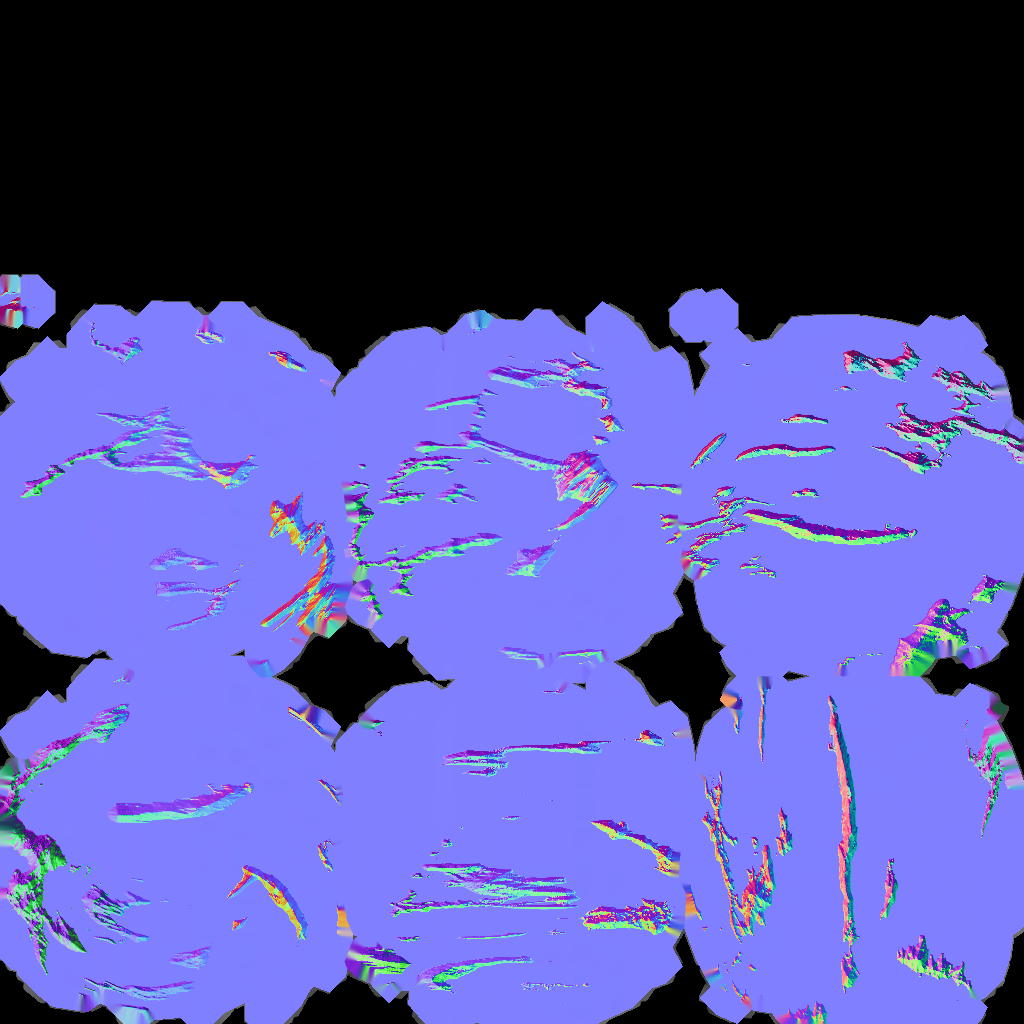
\includegraphics[width=0.4\textwidth]{chapters/11/Images/SteinNormal.png}
    \caption{Eine Abbildung einer Normalmap des Objektes.}
    \label{htl01}
\end{figure}
%todo: abbildung ist highlightet weil ich das geändert habe und das man nachher aufpassen muss dass die nummer stimmt
\noindent Bei der Normal-Map von der \hl{Abbildung 7.3} ist deutlich zu erkennen, dass der blaue Bereich die flache Fläche darstellt, während die farblichen Striche hingegen Kratzer zeigen, welche der Stein beinhaltet.

\subsection{Maps Kombinieren}

Als letzten Schritt müssen alle Maps kombiniert werden. Diese werden in dem Grafikprogramm übereinandergelegt.\\\\
Das Endresultat zeigt den Stein mit einer geringe Polygonanzahl aber mit einer großen Vielfalt an Details. In der nächsten Abbildung wird das Endresultat des Steines gezeigt.

\begin{figure}[H]
    \centering
    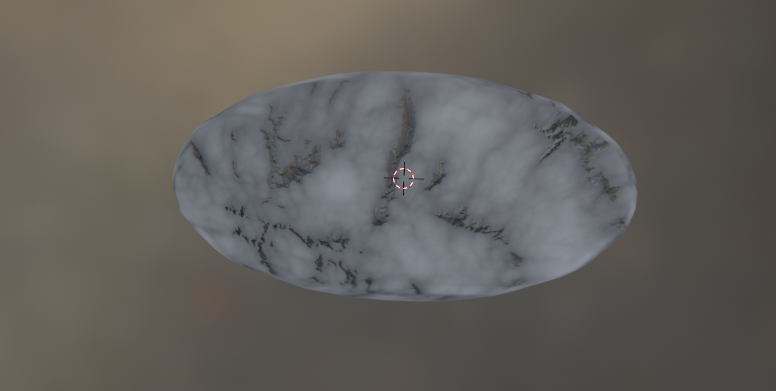
\includegraphics[width=0.6\textwidth]{chapters/11/Images/SteinCombi.png}
    \caption{Eine Abbildung des fertigen Objektes.}
    \label{htl01}
\end{figure}

Um das Objekt in Unity zu implementieren, werden alle Maps in Unity gebraucht. Es ist auch wichtig zu bedenken, dass Unity ein anderes Koordinatensystem hat als Blender. Somit muss beim Export die richtige Richtung angegeben werden. Sonst kann es passieren, dass das Objekt in Unity in eine andere Richtung zeigt.

\begin{figure}[H]
    \centering
    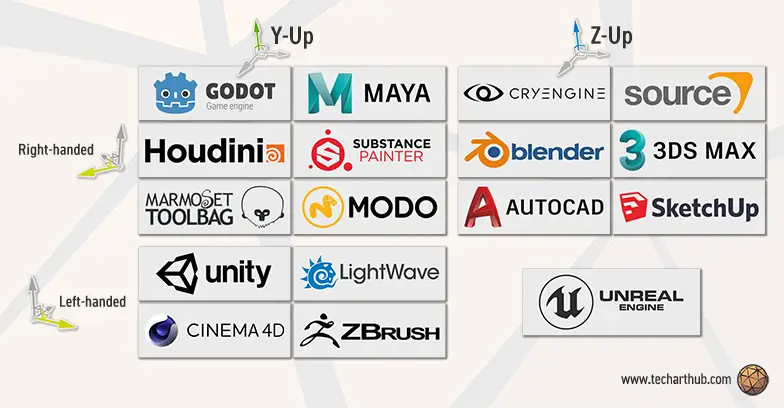
\includegraphics[width=0.6\textwidth]{chapters/11/Images/Koordinaten.png}
    \caption{Eine Abbildung unterschiedlicher Programme und deren Koordinatensystemen}
    \label{htl01}
\end{figure}

\pagebreak